\paragraph{Passing variables}

Functions can also accept the values from variables as concrete values for their parameters. Let's study the following function:

\begin{minipage}[t]{0.45\textwidth}
\vspace{-3pt}
\begin{nllisting}
def twice(text):
    print(text)
    print(text)
fruits = "pineapple blueberry"
twice(fruits)
\end{nllisting}
\end{minipage}
\begin{minipage}[t]{0.45\textwidth}
\vspace{0pt}
\begin{listing}
pineapple blueberry
pineapple blueberry
\end{listing}
\end{minipage}

We passed a single variable called \texttt{fruits} to the function. The value of the variable \texttt{fruits} is passed to the function, where it will now be named \texttt{text}. This \texttt{text} is then printed to the screen twice.

Like before, the order of the values that are passed to a function will determine the parameter names these values get. This is \emph{always} done in order. This is especially important, because sometimes parameters may have the same name as variables found elsewhere in the code. Consider this fragment:

\begin{nnflisting}
x = 10
y = 40
def minus(x, y):
    print(x - y)
minus(y, x)
\end{nnflisting}

Because the values of \texttt{y} and \texttt{x} are passed to the function in that order, inside the function we will have the parameters and their respective values \texttt{x = 40} and \texttt{y = 10}. Hence, the result that is printed will be 30.

\paragraph{Tracing}

Because of the potential confusion between variable and parameter names, we add an explicit step to our function tracing technique: substituting values in the function call. We cross out the variable name and write its value next to it. We can do this before considering the function's definition at all. Now that we have substituted the concrete values, it's easy to copy them into the function call like in earlier sections.

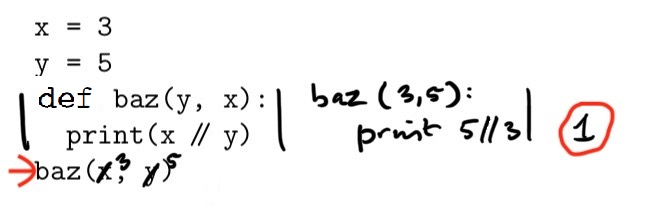
\includegraphics[width=.8\textwidth]{3-trace-varsparams.jpeg}
